%%%%%%%%%%%%%%%%%%%%%%%%%%%%%%%%%%%%%%%%%
% Medium Length Professional CV
% LaTeX Template
% Version 2.0 (8/5/13)
%
% This template has been downloaded from:
% http://www.LaTeXTemplates.com
%
% Original author:
% Trey Hunner (http://www.treyhunner.com/)
%
% Important note:
% This template requires the resume.cls file to be in the same directory as the
% .tex file. The resume.cls file provides the resume style used for structuring the
% document.
%
%%%%%%%%%%%%%%%%%%%%%%%%%%%%%%%%%%%%%%%%%

\documentclass{resume}
\usepackage{hyperref, textcomp, lipsum}
\usepackage{enumitem}
\usepackage[dvipsnames]{xcolor}
\usepackage{graphicx}
\hypersetup{
    colorlinks=true,
    linkcolor=blue,
    filecolor=blue,      
    urlcolor=blue,
}
\usepackage[left=0.5in,top=0.5in,right=0.6in,bottom=0.5in]{geometry}

\name{Darshan Makwana}
\address{\textit{\href{mailto:darshanmakwana412@gmail.com}{darshanmakwana412@gmail.com}} \\ \href{https://github.com/darshanmakwana412}{GitHub} \\ \href{https://www.linkedin.com/in/darshan-makwana-282480228/}{LinkedIn}}
\address{\textbf{WEBPAGE}: \url{https://darshanmakwana412.github.io}}

\begin{document}

\vspace*{0.1in}
\noindent
\begin{minipage}[t]{0.75\textwidth}
My name is Darshan Makwana and I'm a Machine Learning Engineer at \href{https://www.sprinklr.com/}{Sprinklr} currently working on real time voice AI systems and building robust systems for ASR inference. Previously, I was a Research Assistant at \href{https://users.aalto.fi/~kannalj1/}{Aalto Vision Lab} working on 3D Gaussian Splatting and also did research internships at \href{https://www.tum.de/en/}{TU Munich} on quadruped robotics and \href{https://www.hexo.ai/}{Hexo AI} on diffusion models.

\vspace{0.1in}
I graduated from \href{https://www.iitb.ac.in/}{IIT Bombay} with a B.Tech in Mechanical Engineering and Dual Minor in Computer Science and Machine Learning. My interests span computer vision, 3D reconstruction, and efficient ML systems.
\end{minipage}%
\hfill
\begin{minipage}[t]{0.21\textwidth}
\vspace{0pt}
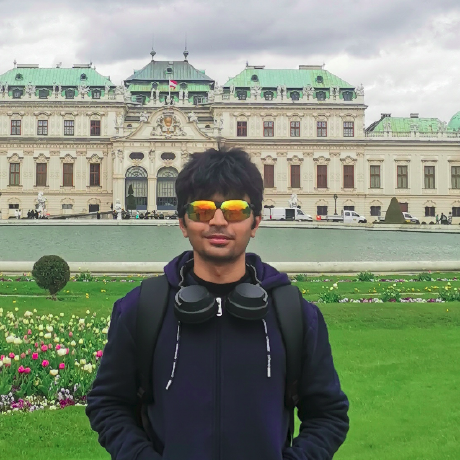
\includegraphics[width=1.1\textwidth]{./../assets/images/bio/darshan1.png}
\end{minipage}
\vspace{0.1in}

\begin{rSection}{Education}
    \vspace*{0.1in}
    
    {\bf Indian Institute of Technology, Bombay} \hfill {2021 - 2025} \\ 
    B.Tech in Mechanical Engineering $|$ Minor in Computer Science and Data Science\\
    Major CPI: 8.82/10 $\cdot$ Minor CPI: 10/10
    
    \begin{itemize}[leftmargin=1.5em, itemsep=0.1em]
    \item \textbf{Team Lead, Inter IIT Tech Meet 13.0} \hfill Dec 2024\\
    {\small Led team of 13 for Adobe deepfake detection challenge to 2nd runner up}
    \item \textbf{Teaching Assistant} \hfill Apr - Jun 2023\\
    {\small PH 112 \& MA 108 $|$ Conducting weekly tutorials and grading assignments for 40+ students}
    \item \textbf{Machine Learning Mentor} \hfill May - Jul 2023\\
    {\small Mentoring 7 students during the summers to pick up pace in ML}
    \item \textbf{Core Team Member, DAV} \hfill Jul 2022 - Apr 2023\\
    {\small Data Analytics Team of the Undergrad Academic Council}
    \item \textbf{Web Coordinator} \hfill May 2022 - Jun 2023\\
    {\small Developed websites for SARC events and alumni portals}
    \end{itemize}
    
    \vspace{0.1in}
    
    {\bf Aalto University, Finland} \hfill {Jan - Jun 2025} \\ 
    Semester Exchange, School of Science\\
    Ranked 3/380+ in Programming Parallel Computers Course\\
    \href{https://darshanmakwana412.github.io/assets/pdfs/ppc_lor.pdf}{Letter of Recommendation}\\
    CPI: 10.0/10.0
    
    \end{rSection}

\begin{rSection}{Experience}
\vspace*{0.1in}

{\bf Sprinklr} {\hfill Gurugram, India}\\
\textit{Machine Learning Engineer (Full-time)} \hfill Aug 2025 - Present\\
Building robust inference serving systems for realtime voice AI applications serving 10M+ monthly voice minutes. Architected changes around whisper to enable 2.5$\times$ increase in throughput with minimal hit on performance. Designed a scheduling strategy for ASR systems achieving 43\% reduction in median E2E latency at high loads (Published at ICLR 2026). 

Built in house MLOps agent for automating deployments, observability and CI/CD pipelines. 

Won 2nd prize in company wide voice hackathon building an end to end voice agent prototype with real time multi-turn conversation handling and tool calling capabilities.

\vspace{0.15in}

{\bf Aalto Vision Lab} {\hfill Helsinki, Finland}\\
\textit{Research Assistant under \href{https://maturk.github.io/}{Matias Turkulainen} \& \href{https://users.aalto.fi/~kannalj1/}{Juho Kannala}} \hfill Jan - Jul 2025\\
Wrote multi GPU training scripts for feedforward gaussian splatting on SLURM clusters. Profiled and optimized training kernels for better GPU utilization. Benchmarked and ablated various optimization techniques for feedforward gaussian splatting.

\vspace{0.15in}

{\bf Sprinklr} {\hfill Gurugram, India}\\
\textit{Product Intern} \hfill May - Jul 2024\\
Benchmarked audio codecs for use in STT and TTS applications. Built a prototype of a unified voice agent for customer support services. Received Pre Placement Offer (PPO).

\vspace{0.15in}

{\bf Technical University of Munich} {\hfill Munich, Germany}\\
\textit{Summer Research Intern $|$ Quadruped Robotics under \href{https://hp-cao.github.io/hongispage/}{Hongpeng Cao} \& \href{https://rtsl.cps.mw.tum.de/personal_page/mcaccamo/}{Marco Cacca}} \hfill Jun - Jul 2023\\
Developed system identification models for dynamics modelling of quadruped robots and implemented MPC based controllers and compared against model free deep RL approaches in simulation.

\vspace{0.15in}

{\bf Hexo AI} {\hfill Remote}\\
\textit{ML Intern $|$ Diffusion Models} \hfill Feb - Apr 2023\\
Open sourced a text conditional latent diffusion model for product photography generation

\vspace{0.15in}

% {\bf 64Squares} {\hfill Remote}\\
% \textit{ML Intern $|$ Contextual Chatbots} \hfill Dec 2022 - Jan 2023\\
% Training and stress testing models for intent and entity extraction via traditional NLP techniques

\end{rSection}

\begin{rSection}{Projects}
\vspace*{0.1in}

% {\bf ThinkMesh} $|$ \href{https://github.com/martianlantern/ThinkMesh}{code} {\small (GitHub $\star$ 274)} \hfill Sep 2025\\
% Parallel reasoning framework for LLMs implementing \href{https://arxiv.org/abs/2203.11171}{Self-Consistency}, \href{https://arxiv.org/abs/1805.00899}{Debate}, \href{https://arxiv.org/abs/2305.10601}{Tree of Thoughts}, and \href{https://arxiv.org/abs/2308.09687}{Graph of Thoughts} strategies with configurable compute budgets.

% \vspace{0.15in}

\noindent
\begin{minipage}[t]{0.8\textwidth}
{\bf Gaussian Masked Autoencoders} $|$ \href{https://github.com/darshanmakwana412/gaussian-mae}{code} \hfill Feb - Mar 2025\\
This is a reproduction of the \href{https://arxiv.org/abs/2501.03229}{Gaussian MAE} paper leveraging Gaussian splats as intermediate latent representation, enabling some zero-shot capabilities.
\end{minipage}%
\hfill
\begin{minipage}[t]{0.15\textwidth}
\vspace{-5pt}
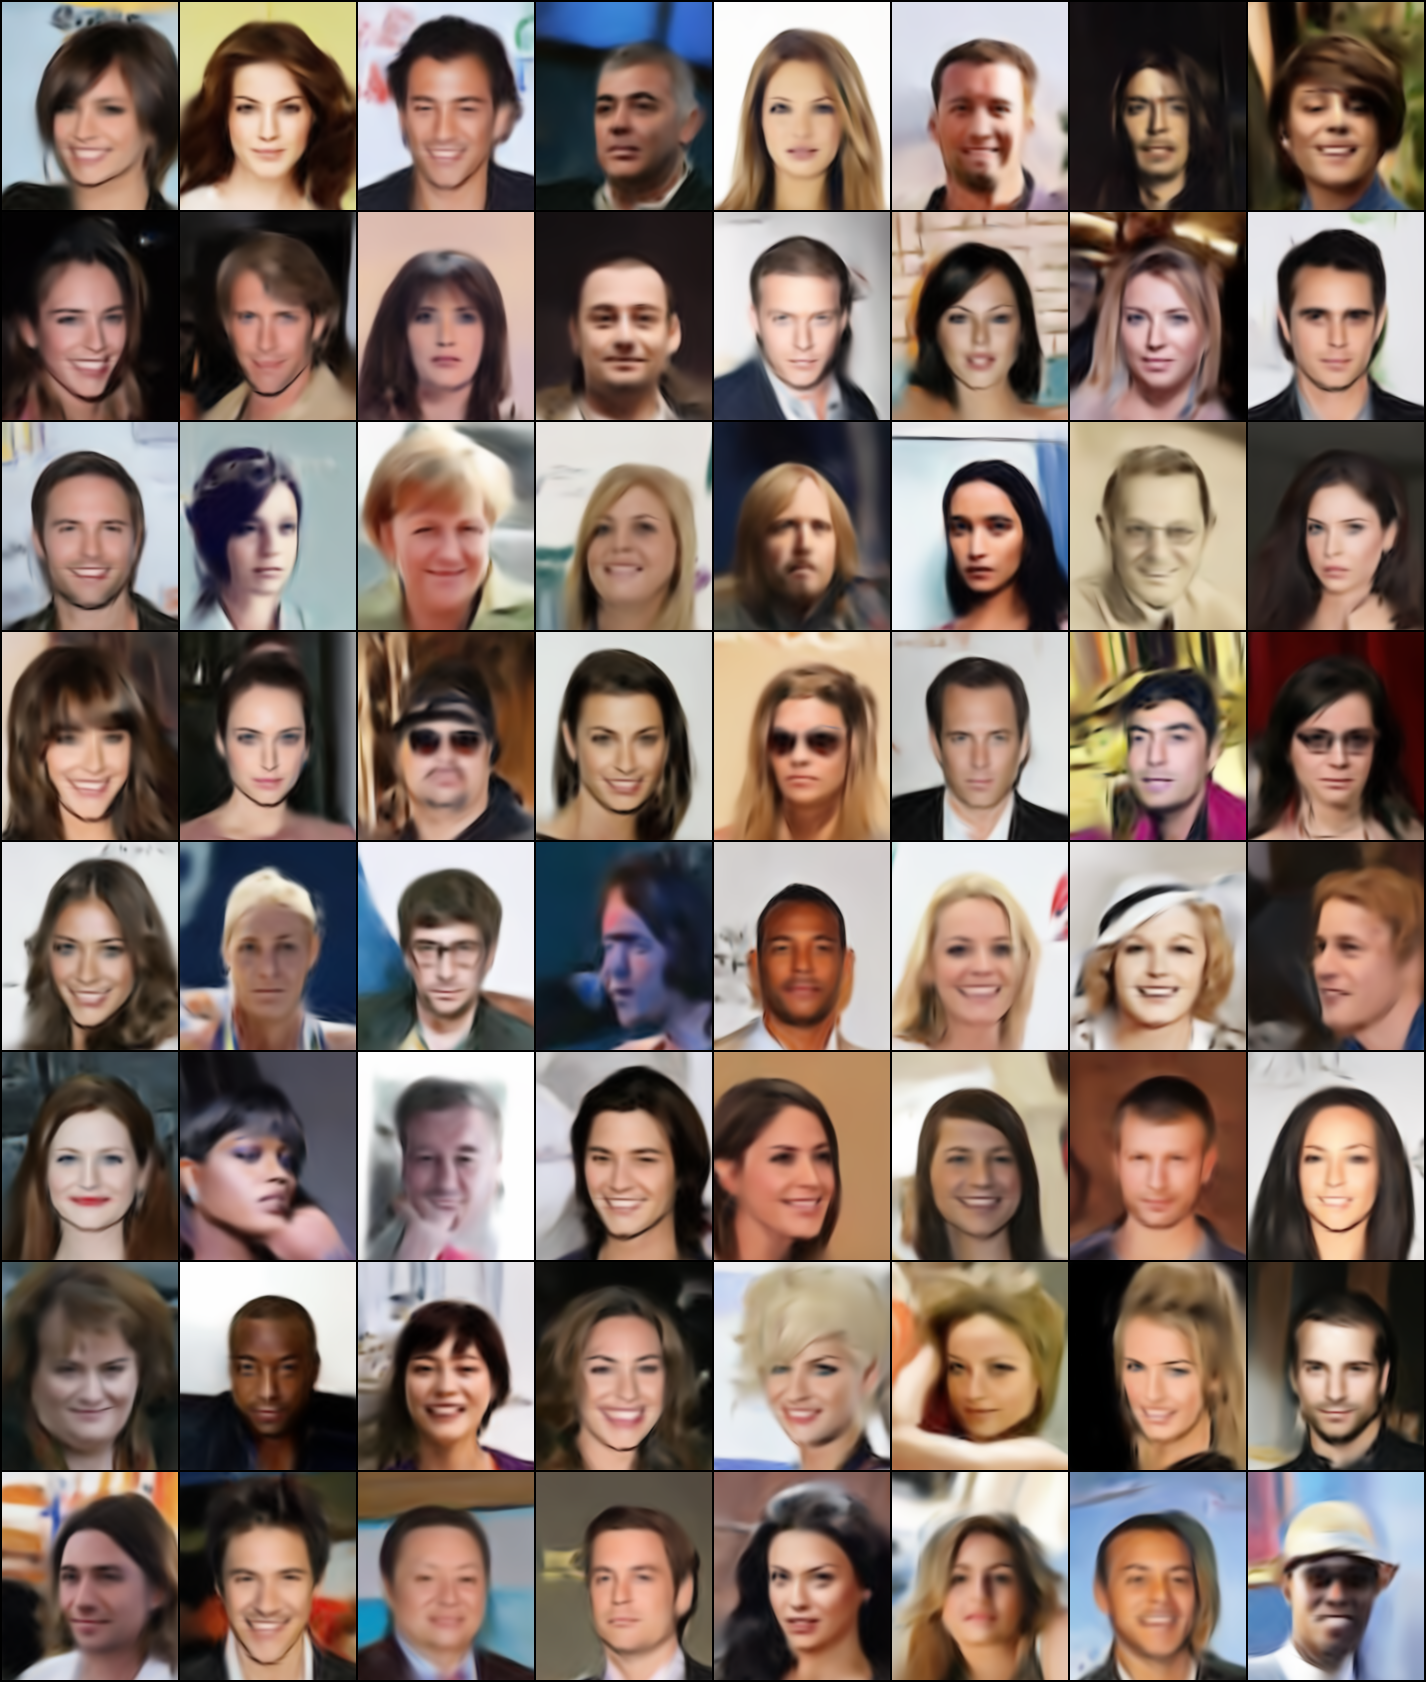
\includegraphics[width=\textwidth]{../assets/images/projects/gmae.png}
\end{minipage}

\vspace{0.15in}

\noindent
\begin{minipage}[t]{0.8\textwidth}
{\bf Minimal 2D Gaussian Splatting} $|$ \href{https://github.com/darshanmakwana412/mings}{code} \hfill Dec 2024\\
A minimal Implementation of gaussian splatting for 2D images using tile based differential rasterizer written in Triton
\end{minipage}%
\hfill
\begin{minipage}[t]{0.15\textwidth}
\vspace{-5pt}
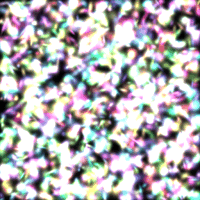
\includegraphics[width=\textwidth]{../assets/images/projects/toucan.png}
\end{minipage}

\vspace{0.15in}

\noindent
\begin{minipage}[t]{0.8\textwidth}
{\bf Multi-View Reconstruction} $|$ \href{https://github.com/darshanmakwana412/Multi_View_Reconstruction}{code} $|$ \href{https://github.com/darshanmakwana412/Multi_View_Reconstruction/blob/main/report.pdf}{report} \hfill Sep - Nov 2024\\
An implementation of volumetrics graph cuts on visual hulls for 3S reconstruction from multiple views. Additionally ray casting for shading is used to render the final scene. This was our final course project for ME 735
\end{minipage}%
\hfill
\begin{minipage}[t]{0.15\textwidth}
\vspace{-5pt}
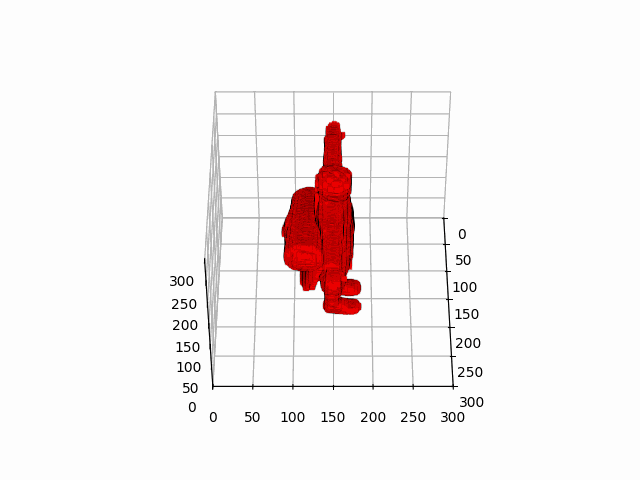
\includegraphics[width=\textwidth]{../assets/images/projects/mvs.png}
\end{minipage}

\vspace{0.15in}

\noindent
\begin{minipage}[t]{0.8\textwidth}
{\bf Structural Optimization} $|$ \href{https://github.com/darshanmakwana412/structure_optimization}{code} $|$ \href{https://github.com/darshanmakwana412/structure_optimization/blob/main/main.pdf}{report} \hfill Jan - Apr 2024\\
A framework for structural optimization of trusses under loading. It uses a matrix formulation of structures and gradient based optimization to compute the optimal spatial configuration of the structure under any loading conditions.
\end{minipage}%
\hfill
\begin{minipage}[t]{0.15\textwidth}
\vspace{-5pt}
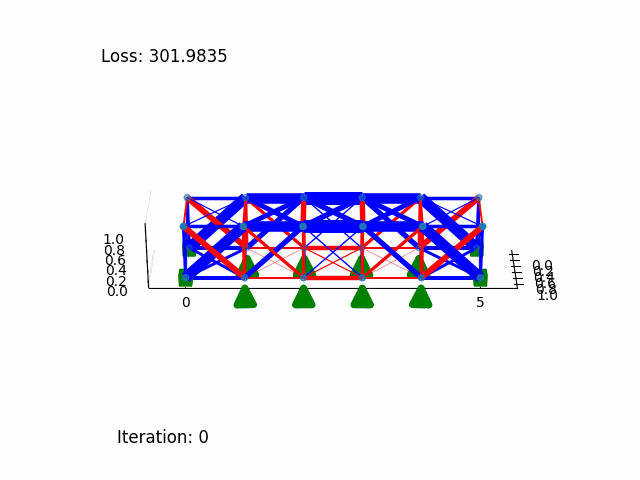
\includegraphics[width=\textwidth]{../assets/images/projects/struct_optim.png}
\end{minipage}

\vspace{0.15in}

\noindent
\begin{minipage}[t]{0.8\textwidth}
{\bf Fractal Curves for Tool Path Planning} $|$ \href{https://github.com/darshanmakwana412/fractal}{code} $|$ \href{https://github.com/darshanmakwana412/fractal/blob/main/draft/tool_path_planning.pdf}{report} \hfill Aug - Nov 2023\\
This is a PoC of using fractal curves for tool path planning in layered 3D printing. It implements a tool path planning algorithm that uses fractal curves via recursive decomposition into smaller fractals, thus the entire layer is a single continuous path.
\end{minipage}%
\hfill
\begin{minipage}[t]{0.15\textwidth}
\vspace{-5pt}
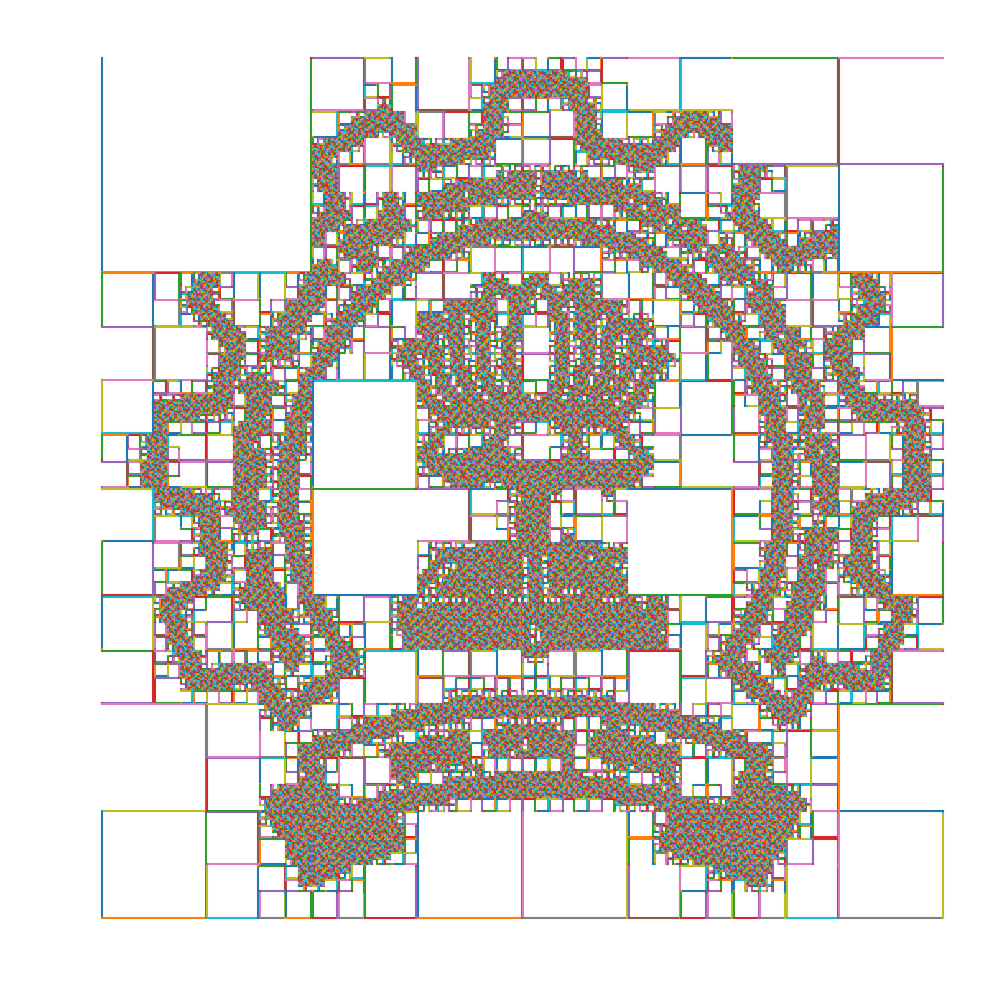
\includegraphics[width=\textwidth]{../assets/images/projects/fractal.png}
\end{minipage}

\end{rSection}

\begin{rSection}{Publications}
\vspace*{0.1in}
{\bf Duration Aware Scheduling for ASR Serving Under Workload Drift} \hfill \href{https://arxiv.org/abs/2603.11273}{CAO @ ICLR 2026}
\textbf{Darshan Makwana}, Yash Jogi, Harsh Kotta, Aayush Kubba.\\

\vspace{0.15in}
{\bf COVID Self diagnosis classification using BERT and LightGBM models} \hfill SMM4H 2023\\
R Chavda, \textbf{Darshan Makwana}, et al.

\end{rSection}

\end{document}
